\documentclass{standalone}
\usepackage{tikz}
\usetikzlibrary{patterns, positioning}
\usepackage[sfdefault]{ClearSans} %% option 'sfdefault' activates Clear Sans as the default text font
\usepackage[T1]{fontenc}

\begin{document}
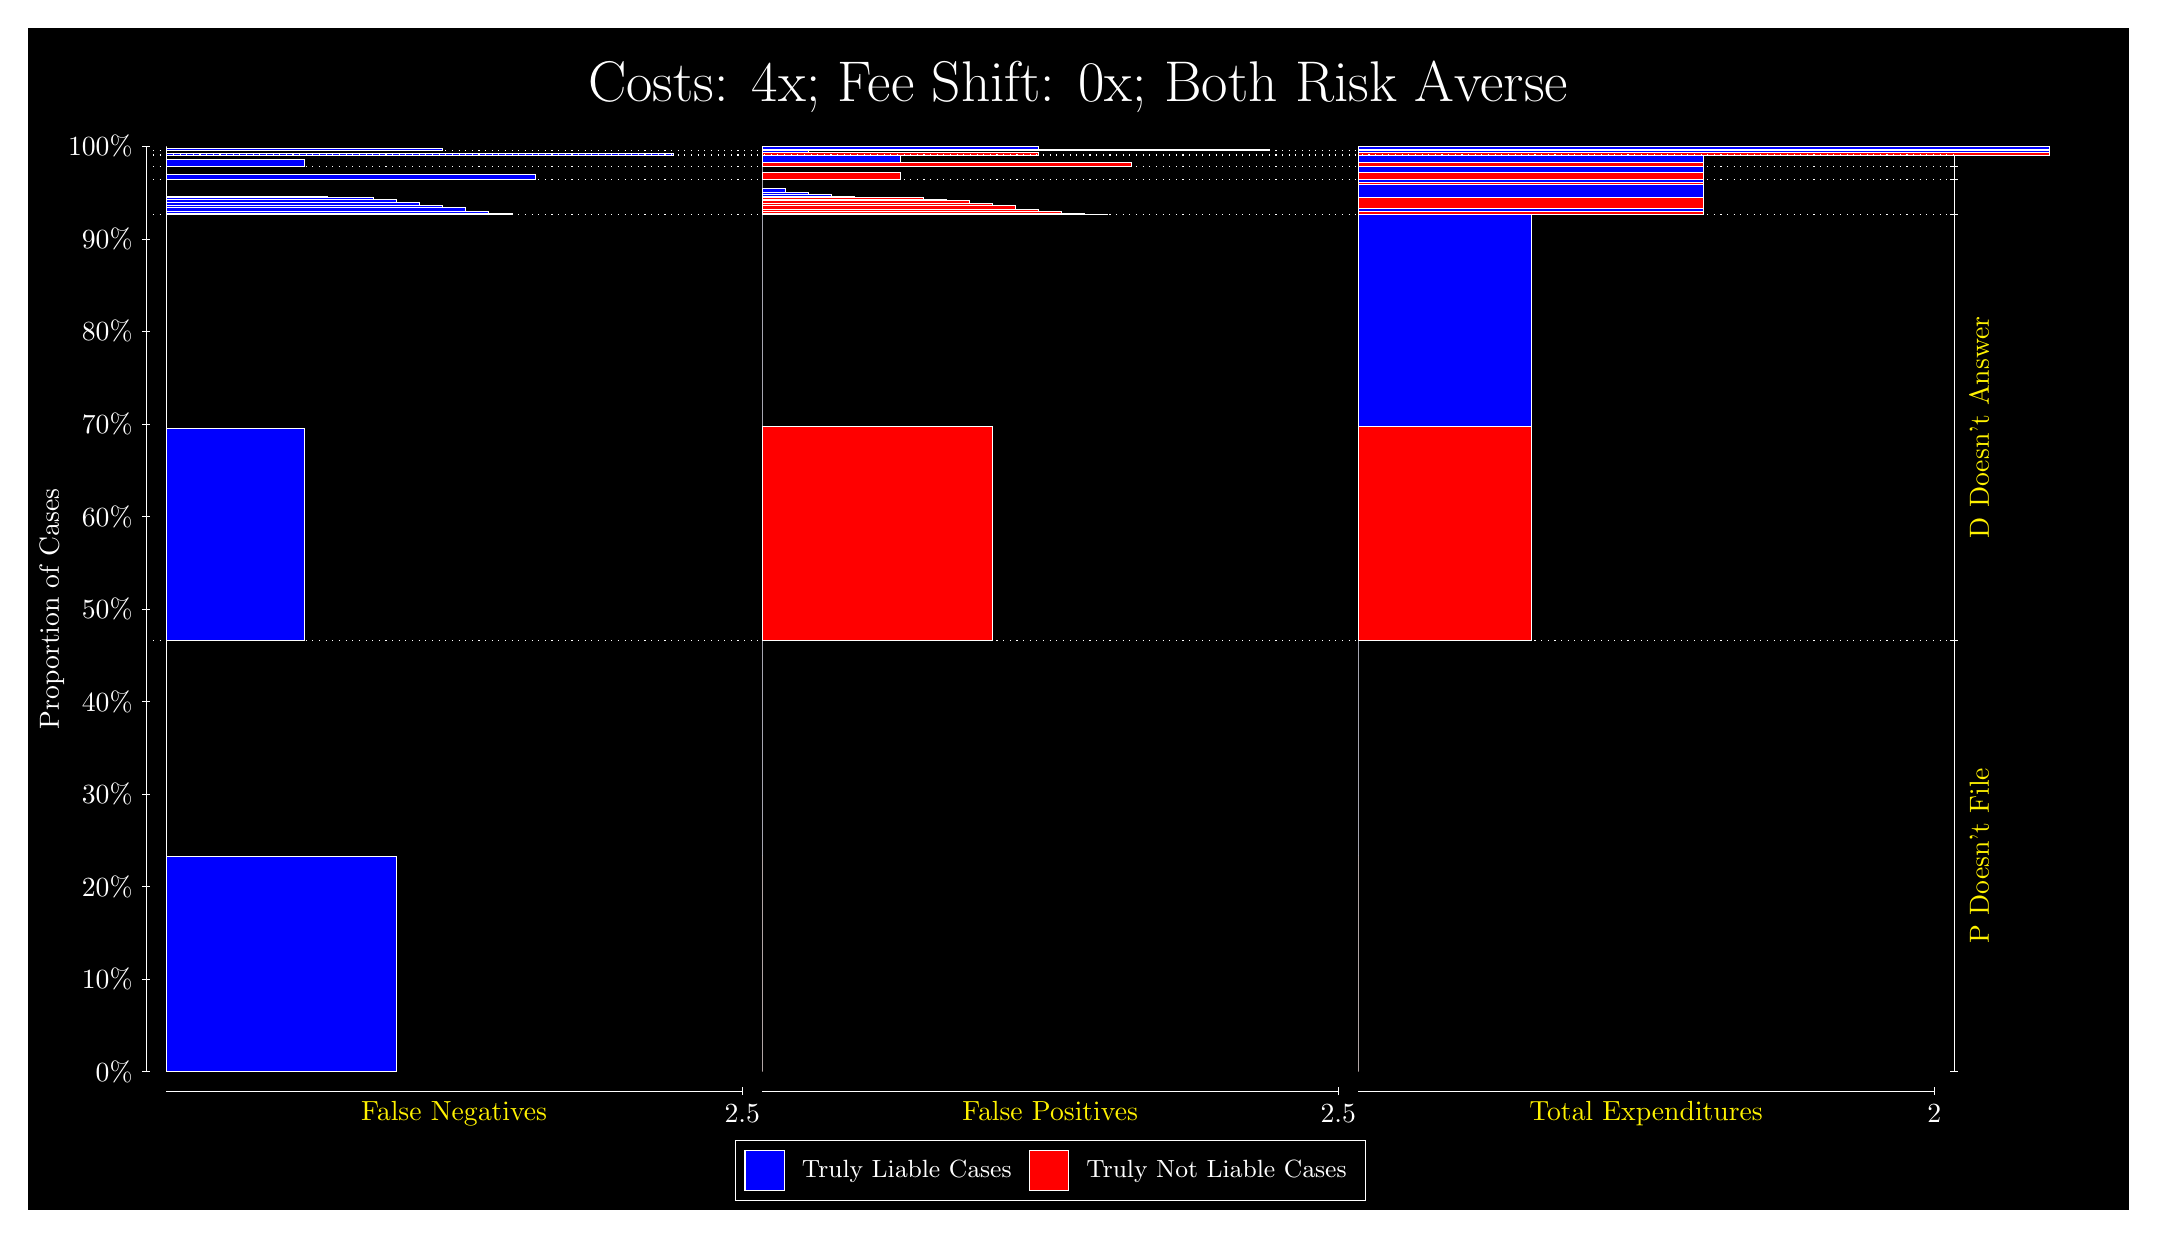
\begin{tikzpicture}
\draw[fill=black] (0,0) rectangle (26.667,15);
\draw[text=white] (0,13.5) rectangle (26.667,15) node[midway] {\huge Costs: 4x; Fee Shift: 0x; Both Risk Averse};
\draw[white, very thin] (1.5,1.75) -- (1.5,13.5);
\node[rotate=90, text=white, anchor=center] at (0.3, 7.625) {Proportion of Cases};
\draw[white, very thin] (1.45,1.75) -- (1.55,1.75);
\node[text=white, anchor=east] at (1.45, 1.75) {0\%};
\draw[white, very thin] (1.45,2.925) -- (1.55,2.925);
\node[text=white, anchor=east] at (1.45, 2.925) {10\%};
\draw[white, very thin] (1.45,4.1) -- (1.55,4.1);
\node[text=white, anchor=east] at (1.45, 4.1) {20\%};
\draw[white, very thin] (1.45,5.275) -- (1.55,5.275);
\node[text=white, anchor=east] at (1.45, 5.275) {30\%};
\draw[white, very thin] (1.45,6.45) -- (1.55,6.45);
\node[text=white, anchor=east] at (1.45, 6.45) {40\%};
\draw[white, very thin] (1.45,7.625) -- (1.55,7.625);
\node[text=white, anchor=east] at (1.45, 7.625) {50\%};
\draw[white, very thin] (1.45,8.8) -- (1.55,8.8);
\node[text=white, anchor=east] at (1.45, 8.8) {60\%};
\draw[white, very thin] (1.45,9.975) -- (1.55,9.975);
\node[text=white, anchor=east] at (1.45, 9.975) {70\%};
\draw[white, very thin] (1.45,11.15) -- (1.55,11.15);
\node[text=white, anchor=east] at (1.45, 11.15) {80\%};
\draw[white, very thin] (1.45,12.325) -- (1.55,12.325);
\node[text=white, anchor=east] at (1.45, 12.325) {90\%};
\draw[white, very thin] (1.45,13.5) -- (1.55,13.5);
\node[text=white, anchor=east] at (1.45, 13.5) {100\%};

\draw[white, very thin] (24.457,1.75) -- (24.457,13.5);
\draw[white, very thin] (24.407,1.75) -- (24.507,1.75);
\node[anchor=west] at (24.407, 1.75) {};
\draw[white, very thin] (24.407,7.2276) -- (24.507,7.2276);
\node[anchor=west] at (24.407, 7.2276) {};
\draw[white, very thin] (24.407,12.634) -- (24.507,12.634);
\node[anchor=west] at (24.407, 12.634) {};
\draw[white, very thin] (24.407,13.079) -- (24.507,13.079);
\node[anchor=west] at (24.407, 13.079) {};
\draw[white, very thin] (24.407,13.244) -- (24.507,13.244);
\node[anchor=west] at (24.407, 13.244) {};
\draw[white, very thin] (24.407,13.39) -- (24.507,13.39);
\node[anchor=west] at (24.407, 13.39) {};
\draw[white, very thin] (24.407,13.447) -- (24.507,13.447);
\node[anchor=west] at (24.407, 13.447) {};
\draw[white, very thin] (24.407,13.5) -- (24.507,13.5);
\node[anchor=west] at (24.407, 13.5) {};

\draw[white, very thin, fill=blue] (1.75,1.75) rectangle (4.6775,4.4888);
\draw[white, very thin, fill=red] (1.75,4.4888) rectangle (1.75,7.2276);
\draw[white, very thin, fill=blue] (1.75,7.2276) rectangle (3.5065,9.9177);
\draw[white, very thin, fill=red] (1.75,9.9177) rectangle (1.75,12.634);
\draw[white, very thin, fill=blue] (1.75,12.634) rectangle (6.1413,12.649);
\draw[white, very thin, fill=blue] (1.75,12.649) rectangle (5.8486,12.671);
\draw[white, very thin, fill=blue] (1.75,12.671) rectangle (5.5558,12.723);
\draw[white, very thin, fill=blue] (1.75,12.723) rectangle (5.2631,12.748);
\draw[white, very thin, fill=blue] (1.75,12.748) rectangle (4.9703,12.791);
\draw[white, very thin, fill=blue] (1.75,12.791) rectangle (4.6775,12.824);
\draw[white, very thin, fill=blue] (1.75,12.824) rectangle (4.3848,12.85);
\draw[white, very thin, fill=blue] (1.75,12.85) rectangle (4.092,12.858);
\draw[white, very thin, fill=blue] (1.75,12.858) rectangle (3.7993,12.866);
\draw[white, very thin, fill=red] (1.75,12.866) rectangle (1.75,13.079);
\draw[white, very thin, fill=blue] (1.75,13.079) rectangle (6.4341,13.148);
\draw[white, very thin, fill=red] (1.75,13.148) rectangle (1.75,13.244);
\draw[white, very thin, fill=blue] (1.75,13.244) rectangle (3.5065,13.338);
\draw[white, very thin, fill=red] (1.75,13.338) rectangle (1.75,13.39);
\draw[white, very thin, fill=blue] (1.75,13.39) rectangle (8.1906,13.409);
\draw[white, very thin, fill=red] (1.75,13.409) rectangle (1.75,13.447);
\draw[white, very thin, fill=blue] (1.75,13.447) rectangle (5.2631,13.479);
\draw[white, very thin, fill=red] (1.75,13.479) rectangle (1.75,13.5);
\draw[white, very thin, fill=red] (9.3189,1.75) rectangle (9.3189,4.4888);
\draw[white, very thin, fill=blue] (9.3189,4.4888) rectangle (9.3189,7.2276);
\draw[white, very thin, fill=red] (9.3189,7.2276) rectangle (12.246,9.9439);
\draw[white, very thin, fill=blue] (9.3189,9.9439) rectangle (9.3189,12.634);
\draw[white, very thin, fill=red] (9.3189,12.634) rectangle (13.71,12.642);
\draw[white, very thin, fill=red] (9.3189,12.642) rectangle (13.417,12.65);
\draw[white, very thin, fill=red] (9.3189,12.65) rectangle (13.125,12.673);
\draw[white, very thin, fill=red] (9.3189,12.673) rectangle (12.832,12.706);
\draw[white, very thin, fill=red] (9.3189,12.706) rectangle (12.539,12.747);
\draw[white, very thin, fill=red] (9.3189,12.747) rectangle (12.246,12.773);
\draw[white, very thin, fill=red] (9.3189,12.773) rectangle (11.954,12.812);
\draw[white, very thin, fill=red] (9.3189,12.812) rectangle (11.661,12.827);
\draw[white, very thin, fill=red] (9.3189,12.827) rectangle (11.368,12.847);
\draw[white, very thin, fill=blue] (9.3189,12.847) rectangle (10.783,12.855);
\draw[white, very thin, fill=blue] (9.3189,12.855) rectangle (10.49,12.863);
\draw[white, very thin, fill=blue] (9.3189,12.863) rectangle (10.197,12.888);
\draw[white, very thin, fill=blue] (9.3189,12.888) rectangle (9.9044,12.922);
\draw[white, very thin, fill=blue] (9.3189,12.922) rectangle (9.6116,12.965);
\draw[white, very thin, fill=blue] (9.3189,12.965) rectangle (9.3189,13.079);
\draw[white, very thin, fill=red] (9.3189,13.079) rectangle (11.075,13.174);
\draw[white, very thin, fill=blue] (9.3189,13.174) rectangle (9.3189,13.244);
\draw[white, very thin, fill=red] (9.3189,13.244) rectangle (14.003,13.296);
\draw[white, very thin, fill=blue] (9.3189,13.296) rectangle (11.075,13.39);
\draw[white, very thin, fill=red] (9.3189,13.39) rectangle (12.832,13.429);
\draw[white, very thin, fill=blue] (9.3189,13.429) rectangle (9.9044,13.447);
\draw[white, very thin, fill=red] (9.3189,13.447) rectangle (15.759,13.468);
\draw[white, very thin, fill=blue] (9.3189,13.468) rectangle (12.832,13.5);
\draw[white, very thin, fill=red] (16.888,1.75) rectangle (16.888,4.4888);
\draw[white, very thin, fill=blue] (16.888,4.4888) rectangle (16.888,7.2276);
\draw[white, very thin, fill=red] (16.888,7.2276) rectangle (19.083,9.9439);
\draw[white, very thin, fill=blue] (16.888,9.9439) rectangle (19.083,12.634);
\draw[white, very thin, fill=red] (16.888,12.634) rectangle (21.279,12.675);
\draw[white, very thin, fill=blue] (16.888,12.675) rectangle (21.279,12.718);
\draw[white, very thin, fill=red] (16.888,12.718) rectangle (21.279,12.858);
\draw[white, very thin, fill=blue] (16.888,12.858) rectangle (21.279,13.013);
\draw[white, very thin, fill=red] (16.888,13.013) rectangle (21.279,13.045);
\draw[white, very thin, fill=blue] (16.888,13.045) rectangle (21.279,13.079);
\draw[white, very thin, fill=red] (16.888,13.079) rectangle (21.279,13.174);
\draw[white, very thin, fill=blue] (16.888,13.174) rectangle (21.279,13.244);
\draw[white, very thin, fill=red] (16.888,13.244) rectangle (21.279,13.296);
\draw[white, very thin, fill=blue] (16.888,13.296) rectangle (21.279,13.39);
\draw[white, very thin, fill=red] (16.888,13.39) rectangle (25.67,13.429);
\draw[white, very thin, fill=blue] (16.888,13.429) rectangle (25.67,13.447);
\draw[white, very thin, fill=red] (16.888,13.447) rectangle (25.67,13.468);
\draw[white, very thin, fill=blue] (16.888,13.468) rectangle (25.67,13.5);
\draw[white, dotted] (1.5,7.2276) -- (24.457,7.2276);
\draw[white, dotted] (1.5,12.634) -- (24.457,12.634);
\draw[white, dotted] (1.5,13.079) -- (24.457,13.079);
\draw[white, dotted] (1.5,13.244) -- (24.457,13.244);
\draw[white, dotted] (1.5,13.39) -- (24.457,13.39);
\draw[white, dotted] (1.5,13.447) -- (24.457,13.447);
\draw[white, very thin] (1.75,1.5) -- (9.0689,1.5);
\node[text=yellow, anchor=north] at (5.4094, 1.5) {False Negatives};
\draw[white, very thin] (9.0689,1.45) -- (9.0689,1.55);
\node[text=white, anchor=north] at (9.0689, 1.45) {2.5};

\draw[white, very thin] (9.3189,1.5) -- (16.638,1.5);
\node[text=yellow, anchor=north] at (12.978, 1.5) {False Positives};
\draw[white, very thin] (16.638,1.45) -- (16.638,1.55);
\node[text=white, anchor=north] at (16.638, 1.45) {2.5};

\draw[white, very thin] (16.888,1.5) -- (24.207,1.5);
\node[text=yellow, anchor=north] at (20.547, 1.5) {Total Expenditures};
\draw[white, very thin] (24.207,1.45) -- (24.207,1.55);
\node[text=white, anchor=north] at (24.207, 1.45) {2};

\node[text=yellow, centered, rotate=90] at (24.777, 4.4888) {P Doesn't File};
\node[text=yellow, centered, rotate=90] at (24.777, 9.9308) {D Doesn't Answer};






\draw (12.978300999999998,1.5) node[draw=none] (baseCoordinate) {};
\begin{scope}[align=center]
        \matrix[scale=0.5, draw=white, below=0.5cm of baseCoordinate, nodes={draw}, column sep=0.1cm]{
            \node[rectangle, draw, minimum width=0.5cm, minimum height=0.5cm, fill=blue] {}; &
            \node[draw=none, font=\small, text=white] (B) {Truly Liable Cases}; &
            \node[rectangle, draw, minimum width=0.5cm, minimum height=0.5cm, fill=red] {}; &
            \node[draw=none, font=\small, text=white] (B) {Truly Not Liable Cases}; \\
            };
\end{scope}

\end{tikzpicture}
\end{document}